\documentclass[9pt,aspectratio=169,xcolor=table]{beamer}

%~~~~~~~~~~~~~~~~~~~~~~~~~~~~~~~~~~~~~~~~~~~~~~~~~~~~~~~~~~~~~~~~~~~~~~~~~~~~~~
% Use roboto Font (recommended)
\usepackage[sfdefault]{roboto}
\usepackage[utf8]{inputenc}
\usepackage[T1]{fontenc}
%~~~~~~~~~~~~~~~~~~~~~~~~~~~~~~~~~~~~~~~~~~~~~~~~~~~~~~~~~~~~~~~~~~~~~~~~~~~~~~

%~~~~~~~~~~~~~~~~~~~~~~~~~~~~~~~~~~~~~~~~~~~~~~~~~~~~~~~~~~~~~~~~~~~~~~~~~~~~~~
% Define where theme files are located. ('/styles')
\usepackage{styles/fluxmacros}
\usefolder{styles}
% Use Flux theme v0.1 beta
% Available style: asphalt, blue, red, green, gray
\usetheme[style=gray]{flux}
%~~~~~~~~~~~~~~~~~~~~~~~~~~~~~~~~~~~~~~~~~~~~~~~~~~~~~~~~~~~~~~~~~~~~~~~~~~~~~~

%~~~~~~~~~~~~~~~~~~~~~~~~~~~~~~~~~~~~~~~~~~~~~~~~~~~~~~~~~~~~~~~~~~~~~~~~~~~~~~
% Extra packages
\usepackage{booktabs}
\usepackage{colortbl}
\usepackage{ragged2e}
\usepackage{amssymb}
\usepackage{multirow}
\usepackage{tikz}
\usetikzlibrary{arrows.meta, positioning, fit, backgrounds, calc, decorations.pathreplacing}
\setbeamertemplate{itemize items}[square]
\usepackage[scaled=.92]{beramono}
\usepackage{listings}
\usepackage{styles/lstlangarm}
\usepackage{array}
\definecolor{bgcolor}{HTML}{F2E9E9}
% lstlangarm.sty references \color{mauve} for string literals but never defines
% it -- only fires when a listing contains a string. Define it here.
\definecolor{mauve}{rgb}{0.58,0,0.82}
% lstlangarm's C style sets commentstyle=green!20, which is unreadable on the
% pink listing background. Darken it globally.
\lstset{commentstyle=\color{green!45!black}}
% ragged-right fixed-width column -- must be defined in the preamble, never
% inside a frame (\newcolumntype's #1 breaks beamer's frame scanner)
\newcolumntype{R}[1]{>{\RaggedRight\arraybackslash}p{#1}}
%~~~~~~~~~~~~~~~~~~~~~~~~~~~~~~~~~~~~~~~~~~~~~~~~~~~~~~~~~~~~~~~~~~~~~~~~~~~~~~
% Table striping: odd rows white, even rows very light gray.
% Needs \documentclass[...,xcolor=table]{beamer} (beamer loads xcolor itself,
% so the option must go on the class, not \usepackage).
\definecolor{stripe}{gray}{0.94}
% \striped makes body rows alternate white, gray, white, ... starting white.
% \rowcolors counts from the first coloured body row; the header is not counted.
\newcommand{\striped}{\rowcolors{1}{white}{stripe}}
%~~~~~~~~~~~~~~~~~~~~~~~~~~~~~~~~~~~~~~~~~~~~~~~~~~~~~~~~~~~~~~~~~~~~~~~~~~~~~~

%~~~~~~~~~~~~~~~~~~~~~~~~~~~~~~~~~~~~~~~~~~~~~~~~~~~~~~~~~~~~~~~~~~~~~~~~~~~~~~
% TikZ block styles -- matches ch1/ch2
% Colour variables are named identically in the book's stm32primer.tex, so any
% tikzpicture using only the \tikzset{...} styles below can be copied verbatim
% between slides and book. Only the \definecolor/\colorlet VALUES differ: the
% book is printed, so it keeps every stroke pure black with muted fills. These
% slides are projected, so both fill AND stroke are bright and saturated to
% grab attention -- see stm32primer.tex for the print palette.
\definecolor{blkfill}{HTML}{DCEBFF}
\definecolor{blkline}{HTML}{1565C0}
\definecolor{accentfill}{HTML}{FFE0B2}
\definecolor{accentline}{HTML}{E65100}
\definecolor{memfill}{HTML}{DFF5DA}
\definecolor{memline}{HTML}{2E7D32}
\definecolor{cellfill}{HTML}{FFFFFF}
\definecolor{cellline}{HTML}{424242}
\definecolor{bitmaskfill}{HTML}{DCEBFF}
\definecolor{bitmaskline}{HTML}{1565C0}
\definecolor{bithitfill}{HTML}{FFE0B2}
\definecolor{bithitline}{HTML}{E65100}
\tikzset{
  blk/.style   = {rectangle, rounded corners=2pt, draw=blkline, fill=blkfill,
                  thick, align=center, font=\small, minimum height=9mm, inner sep=3pt},
  cpublk/.style= {rectangle, rounded corners=2pt, draw=accentline, fill=accentfill,
                  thick, align=center, font=\small\bfseries, minimum height=9mm, inner sep=3pt},
  memblk/.style= {rectangle, rounded corners=2pt, draw=memline, fill=memfill,
                  thick, align=center, font=\small, minimum height=9mm, inner sep=3pt},
  cell/.style  = {rectangle, draw=cellline, fill=cellfill, align=center,
                  font=\normalsize\ttfamily, minimum height=7mm, inner sep=2pt},
  lbl/.style   = {font=\scriptsize, text=Gray},
  flow/.style  = {-{Stealth[length=2mm]}, thick, draw=blkline},
  busline/.style={thick, draw=cellline},
}
% NOTE (theme quirks -- all fail SILENTLY, always page through the PDF):
%  - a second \\ inside a nested {...} group in a TikZ node breaks parsing
%  - {\small ...} wrapped around a nested itemize eats the frame title + list
%  - \usebeamercolor on a [plain] frame falls through to an unstyled default
%  - \newcolumntype inside a frame breaks beamer's frame scanner
%  - lstlisting needs \begin{frame}[fragile]
%  - a TikZ picture wider than its column silently overflows into neighbours
%~~~~~~~~~~~~~~~~~~~~~~~~~~~~~~~~~~~~~~~~~~~~~~~~~~~~~~~~~~~~~~~~~~~~~~~~~~~~~~

%%%%%%%%%%%%%%%%%%%%%%%%%%%%%%%%%%%
%% BEGIN CONDITIONAL COMPILATION %%
%%%%%%%%%%%%%%%%%%%%%%%%%%%%%%%%%%%
\newif\ifwebex
%\webextrue % uncomment to generate section separator
\ifwebex
\AtBeginSection[]{
  \begin{frame}
  \vfill
  \centering
  \begin{beamercolorbox}[sep=8pt,center,shadow=true,rounded=true]{title}
    \usebeamerfont{title}\insertsectionhead\par%
  \end{beamercolorbox}
  \vfill
  \end{frame}
}
\else
\AtBeginSection[]
{
{
    \setbeamercolor{background canvas}{bg=yellow!10}
    \begin{frame}[plain]
        \frametitle{Table of Contents}
        \tableofcontents[currentsection]
    \end{frame}
}
}
\fi
%%%%%%%%%%%%%%%%%%%%%%%%%%%%%%%%%%%
%% END CONDITIONAL COMPILATION   %%
%%%%%%%%%%%%%%%%%%%%%%%%%%%%%%%%%%%

%~~~~~~~~~~~~~~~~~~~~~~~~~~~~~~~~~~~~~~~~~~~~~~~~~~~~~~~~~~~~~~~~~~~~~~~~~~~~~~
% Information
\title{From Digital Systems to Microcontrollers}
\subtitle{\emph{Introduction to ARM Cortex-M Microprocessors} --- Chapter 1}
\author{Mun\'{i}m Zabidi}
\institute{\color{primary}Faculty of Electrical Engineering, Universiti Teknologi Malaysia}
\date{\today}
\titlegraphic{assets/logoutmwhite.png}
%~~~~~~~~~~~~~~~~~~~~~~~~~~~~~~~~~~~~~~~~~~~~~~~~~~~~~~~~~~~~~~~~~~~~~~~~~~~~~~

\begin{document}

\titlepage

\begin{frame}{Table of Contents}
    \tableofcontents
\end{frame}

%===============================================================================
\section{Why This Matters}
%===============================================================================

\begin{frame}{Why This Chapter Matters}
    \leavevmode
    You have built circuits from gates, flip-flops and counters. Each
    circuit did exactly what its \alert{wiring} told it to do. To
    change its behaviour, you had to change the wiring itself.

    \vspace{3mm}
    A microcontroller works differently. It is a digital circuit too,
    but a \alert{program stored in memory} controls its behaviour.

    \vspace{3mm}
    \begin{block}{The same silicon can}
        blink an LED \quad$\cdot$\quad measure a temperature \quad$\cdot$\quad
        drive a motor

        \vspace{1mm}
        \ldots it only depends on the bits you load into it.
    \end{block}

    \vspace{3mm}
    {\small This chapter explains how this is possible.}
\end{frame}

\begin{frame}{Objectives}
    \leavevmode
    {\small After completing this chapter, you should be able to:}

    \vspace{2mm}
    {\small
    \begin{enumerate}\itemsep2pt
        \item Define an embedded system and identify the constraints that
              distinguish embedded design from general-purpose computing.
        \item Distinguish a \alert{microprocessor} from a
              \alert{microcontroller}, and state what each needs to form a
              working system.
        \item Identify the functional units of a CPU --- ALU, control unit,
              decoder, registers --- and state the role of each.
        \item Explain how the address, data and control buses connect the CPU to
              memory and peripherals, and compute the addressable memory of a
              given bus width.
        \item Trace a short program through the fetch--decode--execute cycle,
              stating the contents of each register at every step.
        \item Locate the major blocks of an STM32 microcontroller on a system
              block diagram.
        \item Describe, in outline, how a single C statement becomes a voltage
              change on a physical pin.
    \end{enumerate}}
\end{frame}

\begin{frame}{The One Question}
    \leavevmode
    This chapter introduces many new terms. Every section answers just
    one question. This question is the \alert{thread} that connects
    everything that follows:

    \vspace{4mm}
    \begin{center}
    \fbox{\parbox{.78\textwidth}{\centering\vspace{2mm}
    \large How does a program cause hardware to do something?
    \vspace{2mm}}}
    \end{center}

    \vspace{4mm}
    \begin{block}{The one fact to carry out of this chapter}
        \alert{The CPU has no special instruction for ``turn on an LED''.}

        \vspace{2mm}
        It only has instructions that \alert{read and write memory
        addresses}. Some of these addresses connect not to memory,
        but to hardware instead.

        \vspace{2mm}
        So turning on an LED means \alert{writing a number to an
        address}.
    \end{block}
\end{frame}

\begin{frame}{The Destination}
	\begin{columns}[c]
		% ---- Left: text ----
		\begin{column}{.40\textwidth}
			Before we learn the vocabulary, let us first see where we
			are going.

			\vspace{2mm}
			By the end of this chapter, you will be able to explain
			\alert{every arrow} in this chain. You do not need to
			understand it yet.
		\end{column}
		% ---- Right: flowchart ----
		\begin{column}{.56\textwidth}
			\begin{center}
				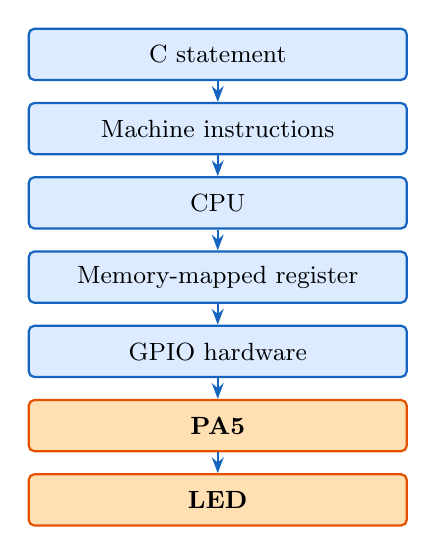
\begin{tikzpicture}[x=10mm, y=8.2mm]
					\foreach \i/\nm in {
						0/{C statement},
						1/{Machine instructions},
						2/{CPU},
						3/{Memory-mapped register},
						4/{GPIO hardware},
						5/{PA5}}{
						\pgfmathtruncatemacro{\isLast}{\i==5}
						\ifnum\isLast=1
						\node[cpublk, minimum width=48mm, minimum height=6.5mm] (n\i) at (0,{-\i*1.15}) {\nm};
						\else
						\node[blk, minimum width=48mm, minimum height=6.5mm] (n\i) at (0,{-\i*1.15}) {\nm};
						\fi
					}
					\foreach \a/\b in {0/1,1/2,2/3,3/4,4/5}{\draw[flow] (n\a) -- (n\b);}
					\node[cpublk, minimum width=48mm, minimum height=6.5mm] (led) at (0,-6.9) {LED};
					\draw[flow] (n5) -- (led);
				\end{tikzpicture}
			\end{center}
		\end{column}
	\end{columns}
\end{frame}

%===============================================================================
\section{Embedded Systems}
%===============================================================================

\begin{frame}{What Makes a System Embedded}
    \begin{columns}[T]
    \begin{column}{.48\textwidth}
        \textbf{General-purpose computer}
        \begin{itemize}
            \item Runs many different applications
            \item The user can program it
            \item \alert{Faster is always better}
            \item Sold on speed, compatibility, price
        \end{itemize}
    \end{column}
    \begin{column}{.48\textwidth}
        \textbf{Embedded system}
        \begin{itemize}
            \item Runs a few functions, fixed at design time
            \item The user cannot program it
            \item Must meet a \alert{fixed deadline}; extra speed may not help
            \item Sold on power, cost, size, \alert{predictability}
        \end{itemize}
    \end{column}
    \end{columns}

    \vspace{3mm}
    \begin{block}{The idea that matters}
        A desktop that answers in 100\,ms instead of 10\,ms is just
        slow. But an airbag controller that fires in 100\,ms instead
        of 10\,ms has \alert{failed}.

        \vspace{1mm}
        Embedded engineering cares about \emph{predictable} time, not
        maximum speed.
    \end{block}
\end{frame}

\begin{frame}{Embedded Systems: An Example}
    \begin{minipage}[c]{0.66\textwidth}
        \includegraphics[width=\textwidth, height=.68\textheight, keepaspectratio]%
            {assets/car-embedded-systems.jpg}
    \end{minipage}%
    \hfill
    \begin{minipage}[c]{0.32\textwidth}
        {\small Each label is at least one \alert{ECU}: an
        \textbf{Electronic Control Unit}. It is a microcontroller, its
        firmware, and a network connection, all together.

        \vspace{2mm}
        A car today carries \textbf{50--150} of these. By
        \textbf{2030}, everyday cars are expected to carry
        \alert{200--250}.

        \vspace{2mm}
        The driver never programs any of them directly.}

        \vspace{3mm}
        {\tiny\color{Gray!80} Diagram credit: Embitel.}
    \end{minipage}

    \vspace{1mm}
    {\scriptsize An ECU is classified by the function it controls: engine control
    module (ECM), body control module (BCM), electronic brake control module
    (EBCM), powertrain control module (PCM), transmission control module (TCM),
    suspension control module (SCM), door control unit (DCM), battery management
    system (BMS), and many more.\par}
\end{frame}

\begin{frame}{SWaP-C}{The constraints that bind}
    \begin{center}
    {\small
    \striped
    \begin{tabular}{@{}l l l@{}}
        \toprule
        \textbf{Constraint} & \textbf{Why it binds} & \textbf{What it forces} \\
        \midrule
        \textbf{S}ize    & Fits inside the product it controls & Package, pin count, board area \\
        \textbf{W}eight  & Portable, airborne, wearable        & Battery size, materials \\
        \textbf{a}nd     &                                     & \\
        \textbf{P}ower   & Battery life, thermal budget        & Clock speed, sleep modes, duty cycle \\
        \textbf{C}ost    & Multiplied by production volume     & Part choice, external components \\
        \bottomrule
    \end{tabular}}
    \end{center}

    \vspace{3mm}
    \begin{block}{Cost is multiplied, not added}
        Saving RM0.50 on one part looks trivial. But at 500{,}000
        units, that saving becomes \alert{RM250{,}000}. This is why
        embedded engineers argue about single resistors.
    \end{block}
\end{frame}

%===============================================================================
\section{Meet the Board}
%===============================================================================
\begin{frame}{From Requirements to Hardware}
	\begin{columns}[c]
		\begin{column}{.48\textwidth}
			\begin{center}
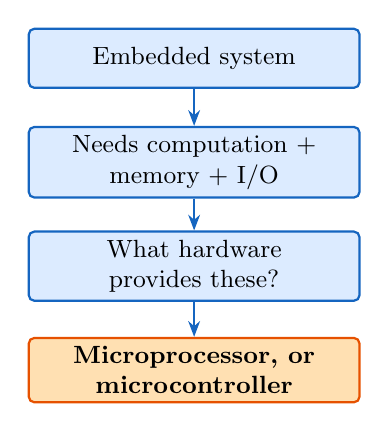
\begin{tikzpicture}[x=10mm, y=8.8mm]
	\node[blk, minimum width=42mm, minimum height=7.5mm] (req)  at (0,4.5) {Embedded system};
	\node[blk, minimum width=42mm, minimum height=7.5mm] (need) at (0,3.0) {Needs computation \(+\)\\memory \(+\) I/O};
	\node[blk, minimum width=42mm, minimum height=7.5mm] (q)    at (0,1.5) {What hardware\\provides these?};
	\node[cpublk, minimum width=42mm, minimum height=7.5mm] (ans) at (0,0.0) {Microprocessor, or\\microcontroller};
	\foreach \a/\b in {req/need, need/q, q/ans}{\draw[flow] (\a) -- (\b);}
\end{tikzpicture}
			\end{center}
		\end{column}
		\begin{column}{.48\textwidth}
			An embedded system is a \emph{requirement}. Something must
			satisfy that requirement.
			\vspace{3mm}
			\begin{block}{The question this raises}
				\centering\alert{What kind of computer belongs inside an embedded system?}
			\end{block}
			\vspace{2mm}
			{\small We will answer this question using one real board,
			so every idea in this chapter has a physical home.}
		\end{column}
	\end{columns}
\end{frame}
\begin{frame}{Meet the Board: STM32 Nucleo-F446RE}
    \begin{columns}[c]
    \begin{column}{.42\textwidth}
        \begin{center}
        \includegraphics[width=\textwidth, height=.6\textheight, keepaspectratio]%
            {assets/nucleo-board.jpg}
        \end{center}
    \end{column}
    \begin{column}{.54\textwidth}
        \textbf{STM32 Nucleo-F446RE}
        {\small
        \begin{itemize}\itemsep1pt
            \item \textbf{ST-LINK} debugger --- the upper third of the
                  board, past the perforation. One USB cable handles
                  power, programming, debugging, and a virtual COM port.
            \item \textbf{USER button} (B1) on \alert{\texttt{PC13}}
            \item \textbf{User LED} (LD2) on \alert{\texttt{PA5}}
        \end{itemize}}

        \vspace{2mm}
        {\small The inner headers follow the Arduino shield layout.
        The outer \textbf{morpho} headers bring out every remaining
        pin.}

        \vspace{2mm}
        {\small \alert{Every blink program in this book drives
        \texttt{PA5}.} Everything we discuss from here on will
        eventually explain this board.}
    \end{column}
    \end{columns}
\end{frame}

%===============================================================================
\section{Inside the Computer}
%===============================================================================

\begin{frame}{Microprocessor and Microcontroller}
    \begin{center}
    {\small
    \striped
    \begin{tabular}{@{}l l l@{}}
        \toprule
        \textbf{Feature} & \textbf{Microprocessor ($\mu$P)} & \textbf{Microcontroller ($\mu$C)} \\
        \midrule
        Integration  & Processor chip only & Processor, RAM, ROM, I/O on one die \\
        Flexibility  & Memory and peripherals scale & Resources fixed inside the chip \\
        Complexity   & Many components, complex PCB & Few components, simple board \\
        Power, cost  & Higher & Optimised for low power and unit cost \\
        Performance  & High clock, heavy computation & Lower clock, control and I/O \\
        \bottomrule
    \end{tabular}}
    \end{center}

    \vspace{3mm}
    \begin{block}{A microprocessor alone is useless}
        It has no RAM, no ROM, and no way to reach the outside world.
        All of this must be wired around it before it can do
        anything. A microcontroller puts exactly this all together on
        one chip. \alert{The Nucleo's chip is a microcontroller}:
        everything on the previous slide sits inside one package.
    \end{block}
\end{frame}

\begin{frame}{Zooming In: From System to Operation}
    \leavevmode
    The next few slides introduce many names at once: buses,
    registers, ALU, decoder. Do not think of this as a list to
    memorise. Instead, think of it as one picture, \alert{zoomed in
    one level at a time}:

    \vspace{2mm}
    \begin{center}
    \begin{tikzpicture}[x=15mm, y=11mm]
        \node[blk,    minimum width=20mm] (sys) at (0,0)   {system};
        \node[cpublk, minimum width=20mm] (cpu) at (1.7,0) {CPU};
        \node[blk,    minimum width=20mm] (reg) at (3.4,0) {register};
        \node[blk,    minimum width=20mm] (ins) at (3.4,-1.1) {instruction};
        \node[blk,    minimum width=20mm] (op)  at (5.1,-1.1) {operation};
        \draw[-{Stealth[length=2mm]}, thick, draw=secondary] (sys.east) -- (cpu.west);
        \draw[-{Stealth[length=2mm]}, thick, draw=secondary] (cpu.east) -- (reg.west);
        \draw[-{Stealth[length=2mm]}, thick, draw=secondary] (reg.south) -- (ins.north);
        \draw[-{Stealth[length=2mm]}, thick, draw=secondary] (ins.east) -- (op.west);
    \end{tikzpicture}
    \end{center}

    \vspace{2mm}
    \begin{block}{Level 1: the whole microcontroller}
        \centering CPU \quad RAM \quad Flash \quad GPIO \quad UART \quad ADC ---
        all on one chip, connected by buses.
    \end{block}

    \vspace{2mm}
    {\small The buses let the CPU \emph{reach} the rest of the chip.
    The registers are what the CPU is \emph{made of}. Both sit one
    level deeper than ``the microcontroller.''}
\end{frame}

\begin{frame}{The Three Buses}

\begin{center} 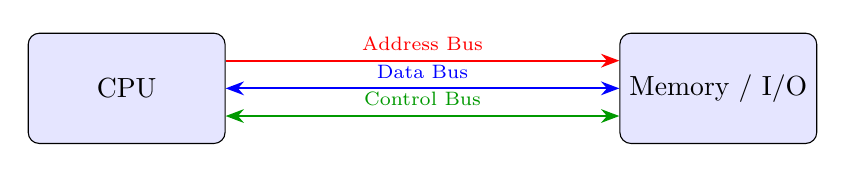
\begin{tikzpicture}[ >=Stealth, bus/.style={thick}, block/.style={draw, rounded corners, minimum width=2.5cm, minimum height=14mm, fill=blue!10} ] \node[block] (cpu) {CPU}; \node[block, right=5cm of cpu] (mem) {Memory / I/O};
		% Address bus
		\draw[->, red, bus] ([yshift=10pt]cpu.east) -- node[above] {\scriptsize Address Bus} ([yshift=10pt]mem.west);
		% Data bus
		\draw[<->, blue, bus] (cpu.east) -- node[above] {\scriptsize Data Bus} (mem.west);
		% Control bus
		\draw[<->, green!60!black, bus] ([yshift=-10pt]cpu.east) -- node[above] {\scriptsize Control Bus} ([yshift=-10pt]mem.west); \end{tikzpicture} \end{center}
    \begin{center}
    {\small
    \striped
    \begin{tabular}{@{}l l l@{}}
        \toprule
        \textbf{Bus} & \textbf{Direction} & \textbf{Carries} \\
        \midrule
        \textbf{Address} & Unidirectional, CPU $\rightarrow$ device
            & \emph{Which} location. Width sets the addressable range \\
        \textbf{Data}    & Bidirectional
            & \emph{What} value. Width sets how much moves per transfer \\
        \textbf{Control} & Bidirectional
            & \emph{When} and \emph{what kind}: read/write, timing, interrupts \\
        \bottomrule
    \end{tabular}}
    \end{center}

    \vspace{3mm}
    \begin{block}{Address width sets the memory map}
        $2^{n}$ addressable bytes for an $n$-bit address bus.

        \vspace{1mm}
        $2^{16} = 64$\,KB \quad$\cdot$\quad $2^{20} = 1$\,MB \quad$\cdot$\quad
        $2^{32} = \alert{4\,\text{GB}}$: the Cortex-M4
    \end{block}

    \vspace{2mm}
    {\small \textbf{You already know this:} an address is the input
    to a \alert{decoder}. It works the same way as the one-of-$N$
    selection you built with a 3-to-8 decoder, just at a much larger
    scale.}

\end{frame}


\begin{frame}{Using the Buses: Fetching an Instruction}
    \leavevmode
    Suppose the CPU needs the instruction stored at \texttt{0x1000}:

    \vspace{2mm}
    \begin{center}
    {\small
    \begin{tabular}{@{}l l@{}}
        \toprule
        \textbf{Bus} & \textbf{Carries, this step} \\
        \midrule
        Address bus & \texttt{0x1000} --- CPU asks for this location \\
        Control bus & \texttt{READ} --- CPU asserts a read \\
        Memory      & responds with \texttt{LOAD 0x2000} \\
        Data bus    & carries that instruction back to the CPU \\
        \bottomrule
    \end{tabular}}
    \end{center}
\begin{center} 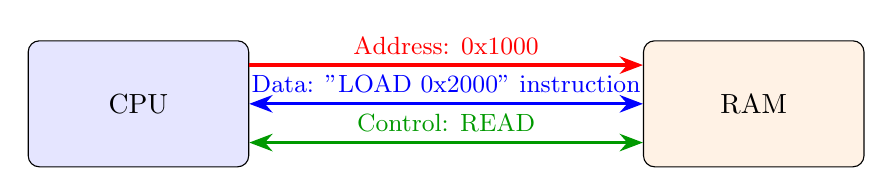
\begin{tikzpicture}[ >=Stealth, block/.style={draw, rounded corners, minimum width=2.8cm, minimum height=1.6cm} ] \node[block, fill=blue!10] (cpu) {CPU}; \node[block, fill=orange!10, right=5cm of cpu] (ram) {RAM}; \draw[->, very thick, red] ([yshift=14pt]cpu.east) -- node[above] {\small Address: 0x1000} ([yshift=14pt]ram.west); \draw[<->, very thick, blue] (cpu.east) -- node[above] {\small Data: "LOAD 0x2000" instruction} (ram.west); \draw[<->, very thick, green!60!black] ([yshift=-14pt]cpu.east) -- node[above] {\small Control: READ} ([yshift=-14pt]ram.west); \end{tikzpicture} \end{center}
    \vspace{1mm}
    \begin{block}{The same pattern repeats for every data access}
        The address bus names the location. The control bus says read
        or write. The data bus carries the value. \alert{Three buses,
        one transaction.} We will use this exact pattern again when we
        trace a program.
    \end{block}
\end{frame}

\begin{frame}[plain]{Zoom 2: Inside the CPU}
    \begin{center}
    \includegraphics[width=.88\textwidth, height=.72\textheight, keepaspectratio]%
        {assets/cpu_inside.pdf}
    \end{center}

    \vspace{1mm}
    {\small\centering The registers in the centre connect to memory.
    The decoder, control unit and ALU on the left have \alert{no
    direct memory access}. Everything they touch must first pass
    through a register.\par}
\end{frame}

\begin{frame}{Zoom 3: The Registers That Matter}
    \leavevmode
    Five names appear on the previous diagram. Not all of them need
    the same amount of attention yet:

    \vspace{2mm}
    \begin{columns}[T]
    \begin{column}{.48\textwidth}
        \textbf{Must understand now}
        \begin{itemize}
            \item \textbf{PC} --- address of the \alert{next} instruction
            \item \textbf{IR} --- the instruction just fetched
            \item \textbf{ACC} --- operand and result of the ALU
        \end{itemize}
    \end{column}
    \begin{column}{.48\textwidth}
        \textbf{Can recognise, needn't memorise yet}
        \begin{itemize}
            \item \textbf{AR} --- address of the data being accessed
            \item \textbf{DR} --- value in transit to or from that address
        \end{itemize}
    \end{column}
    \end{columns}

    \vspace{3mm}
    \begin{block}{Why ``no direct memory access'' matters}
        This is why \alert{load/store} architectures exist. On the
        Cortex-M4, you cannot add two values that sit in memory
        directly. You must \texttt{LDR} them into registers,
        \texttt{ADD} them, then \texttt{STR} the result back. Chapters
        5--7 explain this idea in more detail.
    \end{block}

    \vspace{2mm}
    {\small Chapter 2 replaces this generic register set with the
    Cortex-M4's actual sixteen registers. For now, just keep this
    simple picture in mind.}
\end{frame}

%===============================================================================
\section{Tracing z = x + y}
%===============================================================================

\begin{frame}{One Line of C, Traced in Hardware}
    \leavevmode
    Consider the simplest possible program:

    \vspace{2mm}
    \begin{center}\texttt{z = x + y;}\end{center}

    \vspace{2mm}
    \begin{block}{We will use this one line to discover what a CPU actually does}
        One line of C becomes three machine instructions. Every
        register and operation from the last few slides gets a
        \alert{job} to do in making this happen.
    \end{block}

    \vspace{3mm}
    \begin{columns}[T]
    \begin{column}{.46\textwidth}
        \textbf{Program memory}
        \begin{center}
        {\small
        \striped
        \begin{tabular}{@{}l l@{}}
            \toprule
            \textbf{Address} & \textbf{Instruction} \\
            \midrule
            \texttt{0x1000} & \texttt{LOAD~ 0x2000} \\
            \texttt{0x1002} & \texttt{ADD~~ 0x2002} \\
            \texttt{0x1004} & \texttt{STORE 0x2004} \\
            \bottomrule
        \end{tabular}}
        \end{center}
    \end{column}
    \begin{column}{.46\textwidth}
        \textbf{Data memory}
        \begin{center}
        {\small
        \striped
        \begin{tabular}{@{}l l@{}}
            \toprule
            \textbf{Address} & \textbf{Value} \\
            \midrule
            \texttt{0x2000} & \texttt{1} \\
            \texttt{0x2002} & \texttt{2} \\
            \texttt{0x2004} & \texttt{?} \\
            \bottomrule
        \end{tabular}}
        \end{center}
    \end{column}
    \end{columns}
\end{frame}

\begin{frame}{Six Questions, Six Answers}
    \leavevmode
    Each new concept earns its place here by answering one question
    in this trace:

    \vspace{3mm}
    \begin{center}
    {\small
    \begin{tabular}{@{}c l l@{}}
        \toprule
        & \textbf{Question} & \textbf{Answer} \\
        \midrule
        1 & What is \texttt{x}? & value at \texttt{0x2000} \\
        2 & How does the CPU obtain it? & \texttt{LOAD} \\
        3 & Where does it go? & \texttt{ACC} \\
        4 & How does addition happen? & the \texttt{ALU} \\
        5 & Where does the result go? & \texttt{ACC} \\
        6 & How does it become \texttt{z}? & \texttt{STORE} \\
        \bottomrule
    \end{tabular}}
    \end{center}

    \vspace{3mm}
    \begin{block}{This is much easier to remember than a list}
        ``Here are five registers, memorise what they do'' gives
        these concepts no real job to do. \alert{Every concept in the
        next three slides appears here because this trace needs it.}
    \end{block}
\end{frame}

%===============================================================================
\section{The Instruction Execution Cycle}
%===============================================================================

\begin{frame}{The CPU Has an Instruction. Now What?}
    \leavevmode
    \begin{center}
    \fbox{\parbox{.8\textwidth}{\centering\vspace{2mm}
    The CPU has fetched an instruction. What does it actually do with it?
    \vspace{2mm}}}
    \end{center}

    \vspace{4mm}
    \begin{center}
    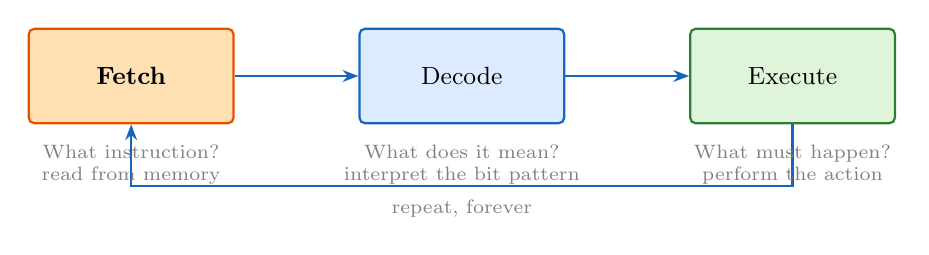
\begin{tikzpicture}[x=10mm, y=10mm]
        \node[cpublk, minimum width=26mm, minimum height=12mm] (f) at (0,0)   {Fetch};
        \node[blk,    minimum width=26mm, minimum height=12mm] (d) at (4.2,0) {Decode};
        \node[memblk, minimum width=26mm, minimum height=12mm] (e) at (8.4,0) {Execute};
        \draw[flow] (f) -- (d);
        \draw[flow] (d) -- (e);
        \draw[flow] (e.south) -- (8.4,-1.4) -- (0,-1.4) -- (f.south);
        \node[lbl, anchor=north] at (4.2,-1.45) {repeat, forever};
        \node[lbl, anchor=north, align=center] at (0,-0.75)   {What instruction?\\read from memory};
        \node[lbl, anchor=north, align=center] at (4.2,-0.75) {What does it mean?\\interpret the bit pattern};
        \node[lbl, anchor=north, align=center] at (8.4,-0.75) {What must happen?\\perform the action};
    \end{tikzpicture}
    \end{center}

    \vspace{2mm}
    {\small This is a finite state machine, driven by the clock. You
    built FSMs in digital electronics. \alert{A CPU is the largest one
    you have met so far.} The loop never stops while the machine has
    power. This is why an embedded program's \texttt{main()} is an
    infinite loop \emph{by design}.}
\end{frame}

\begin{frame}[plain]{Executing \texttt{LOAD 0x2000}}
    \begin{center}
    \includegraphics[width=.82\textwidth, height=.74\textheight, keepaspectratio]%
        {assets/cpu_load.pdf}
    \end{center}
    \vspace{1mm}
    {\small\centering The value \texttt{1} at address \texttt{0x2000}
    reaches the Accumulator. This answers questions 1--3 of the trace.
    Note step \textbf{6}: the \alert{PC increases during decode}, not
    after execute.\par}
\end{frame}

\begin{frame}[plain]{Executing \texttt{ADD 0x2002}}
    \begin{center}
    \includegraphics[width=.82\textwidth, height=.74\textheight, keepaspectratio]%
        {assets/cpu_add.pdf}
    \end{center}
    \vspace{1mm}
    {\small\centering The value \texttt{2} is fetched, and the
    \alert{ALU} adds it to the Accumulator. The Accumulator becomes
    \texttt{3}. This answers questions 4 and 5.\par}
\end{frame}

\begin{frame}[plain]{Executing \texttt{STORE 0x2004}}
    \begin{center}
    \includegraphics[width=.82\textwidth, height=.74\textheight, keepaspectratio]%
        {assets/cpu_store.pdf}
    \end{center}
    \vspace{1mm}
    {\small\centering The Accumulator's \texttt{3} is written out to
    \texttt{0x2004}. This answers question 6. The program is now
    complete: three instructions, each made of several internal
    operations.\par}
\end{frame}

%===============================================================================
\section{From C to a Pin}
%===============================================================================

\begin{frame}{We Can Now Answer the Question We Started With}
    \leavevmode
    \begin{center}
    \fbox{\parbox{.7\textwidth}{\centering\vspace{2mm}
    \large How does a program cause hardware to do something?
    \vspace{2mm}}}
    \end{center}

    \vspace{3mm}
    {\small We just traced \texttt{z = x + y;} through LOAD, ADD, and
    STORE. These were all ordinary memory addresses, nothing more.
    Now let us return to the board: what happens when the address is
    not a memory cell, but a peripheral instead?}
\end{frame}

\begin{frame}[fragile]{One Line of C, Back on the Board}
    \begin{columns}[c]
    \begin{column}{.46\textwidth}
        Look at this line. It appears in almost every STM32 program ever
        written:

        \vspace{2mm}
\begin{lstlisting}[language=C, basicstyle=\ttfamily\normalsize]
GPIOA->ODR |= (1U << 5);
\end{lstlisting}

        \vspace{2mm}
        {\small You already know every symbol here: a pointer, a
        structure member, a compound bitwise-OR assignment, and a
        left shift.}

        \vspace{2mm}
        {\small What may not be obvious is that running this one
        statement \alert{turns on an LED}: the LED on \texttt{PA5},
        on the board you met at the start of this chapter.}
    \end{column}
    \begin{column}{.5\textwidth}
        \begin{center}
        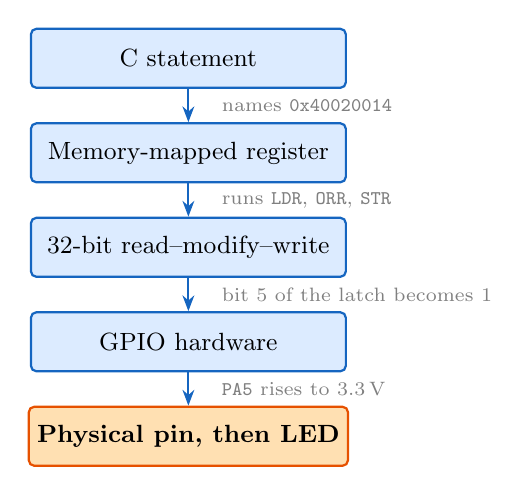
\begin{tikzpicture}[x=10mm, y=10mm]
            \node[blk,    minimum width=40mm, minimum height=7.5mm] (c)   at (0,2.4)  {C statement};
            \node[blk,    minimum width=40mm, minimum height=7.5mm] (reg) at (0,1.2)  {Memory-mapped register};
            \node[blk,    minimum width=40mm, minimum height=7.5mm] (rmw) at (0,0.0)  {32-bit read--modify--write};
            \node[blk,    minimum width=40mm, minimum height=7.5mm] (hw)  at (0,-1.2) {GPIO hardware};
            \node[cpublk, minimum width=40mm, minimum height=7.5mm] (pin) at (0,-2.4) {Physical pin, then LED};
            \foreach \a/\b in {c/reg, reg/rmw, rmw/hw, hw/pin}{\draw[flow] (\a) -- (\b);}
            \node[lbl, anchor=west] at (0.3,1.8)  {names \texttt{0x40020014}};
            \node[lbl, anchor=west] at (0.3,0.6)  {runs \texttt{LDR}, \texttt{ORR}, \texttt{STR}};
            \node[lbl, anchor=west] at (0.3,-0.6) {bit 5 of the latch becomes 1};
            \node[lbl, anchor=west] at (0.3,-1.8) {\texttt{PA5} rises to 3.3\,V};
        \end{tikzpicture}
        \end{center}
    \end{column}
    \end{columns}
\end{frame}

\begin{frame}{The Bookend}
    \leavevmode
    \begin{block}{The CPU still does not know what an LED is}
        It only knows how to execute instructions and access
        addresses. Every step in that chain was ordinary: the same
        \texttt{LDR}/\texttt{ORR}/\texttt{STR} pattern as any other
        read-modify-write.
    \end{block}

    \vspace{4mm}
    \begin{center}
    \fbox{\parbox{.78\textwidth}{\centering\vspace{2mm}
    \large Turning on an LED is writing a number to an address.
    \vspace{2mm}}}
    \end{center}

    \vspace{2mm}
    {\small This is the same sentence from ``The One Question.'' Now
    you fully understand it.}
\end{frame}

\begin{frame}{Summary: The Causal Chain}
	\begin{columns}[c]
		% ---- Left: flowchart ----
		\begin{column}{.58\textwidth}
			\begin{center}
				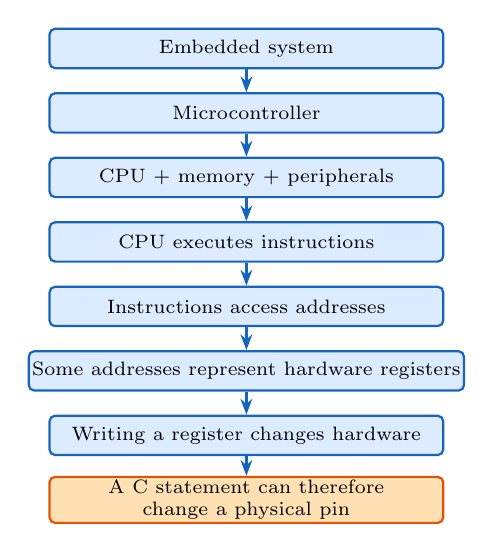
\begin{tikzpicture}[x=10mm, y=7.8mm]
					\foreach \i/\nm in {
						0/{Embedded system},
						1/{Microcontroller},
						2/{CPU + memory + peripherals},
						3/{CPU executes instructions},
						4/{Instructions access addresses},
						5/{Some addresses represent hardware registers},
						6/{Writing a register changes hardware}}{
						\node[blk, minimum width=50mm, minimum height=5.0mm, inner sep=1.2pt,
						font=\scriptsize] (n\i) at (0,{-\i*1.05}) {\nm};
					}
					\node[cpublk, minimum width=50mm, minimum height=5.0mm, inner sep=1.2pt,
					font=\scriptsize] (n7) at (0,-7.35)
					{A C statement can therefore\\change a physical pin};
					\foreach \a/\b in {0/1,1/2,2/3,3/4,4/5,5/6,6/7}{\draw[flow] (n\a) -- (n\b);}
				\end{tikzpicture}
			\end{center}
		\end{column}
		% ---- Right: terminology ----
		\begin{column}{.38\textwidth}
			{\scriptsize
				\textbf{Terminology covered}\\[1mm]
				\begin{itemize}
					\item Embedded systems and SWaP-C
					\item Microprocessor vs microcontroller
					\item Buses
					\item CPU registers, ALU, control unit
					\item Fetch--decode--execute
					\item Memory-mapped I/O
				\end{itemize}
				\vspace{3mm}
				\textbf{Next: Chapter 2}\\[1mm]
				Turns this generic CPU into the specific one on your
				bench.}
		\end{column}
	\end{columns}
\end{frame}

%===============================================================================
\section{Design Challenge}
%===============================================================================

\begin{frame}{Design Challenge}{To be worked on paper, before any code}
    \leavevmode
    {\small You now know enough architecture to reason about this
    design before choosing a microcontroller.}

    \vspace{1mm}
    \begin{block}{The brief}
        A portable \alert{water-quality logger} must:
        \begin{itemize}
            \item run for \textbf{one year} on a coin cell
            \item record a measurement every \textbf{15 minutes}
            \item survive being \textbf{dropped in a river}
            \item cost under \textbf{\$40} in quantities of 500
        \end{itemize}
    \end{block}

    \vspace{2mm}
    \textbf{Do not choose a specific part number.} Instead:
    \begin{enumerate}\itemsep0pt
        \item Identify which \alert{SWaP-C} constraint binds hardest
              here.
        \item Explain what this one constraint forces to be true about
              the \textbf{processor}, the \textbf{memory}, and the
              \textbf{duty cycle}.
        \item State one requirement you would go back and \alert{question
              with the customer}, and explain why.
    \end{enumerate}

    \vspace{1mm}
    {\scriptsize SWaP-C \(\to\) architecture \(\to\) memory \(\to\) duty cycle
    \(\to\) processor requirements: the same chain this chapter just
    built, now applied to a new system.}
\end{frame}

\begin{frame}[plain]
    \begin{center}
        \vfill
        {\usebeamerfont{title}\color{primary}\Huge Questions?}
        \vfill
        {\small\color{Gray} \emph{Introduction to ARM Cortex-M Microprocessors} --- Chapter 1}
        \vfill
    \end{center}
\end{frame}

\end{document}
